\section{Methods}\label{sec:methods}

\subsection{Dataset}

The data used for this paper originates from the 'Monitoring error-related potentials' dataset, created by \cite{chavarriaga2010learning}. This dataset is publically available on the BCNI Horizon 2020 project website. For this experiment, users were placed in front of a screen where they had to observe a moving cursor. The working area of the screen consisted of 20 locations along the horizontal plane. A coloured square would appear on the cursor's left or right side. This square indicates the target the cursor should move towards. At each trial, the cursor would move along the horizontal axis towards the target. Once the target has been reached, the cursor will stay in place, and a new target will appear along the horizontal plane, no more than three positions away from the cursor.

During the experiments, users were asked to solely monitor the agent's performance, knowing the goal of reaching the target. They had no control over the cursor. At each trial, there was a 20\% chance for the cursor to move in the opposite direction relative to the target, which contradicts the agent's goal. These trials indicate a different outcome than the participant anticipated for an 'Error Related Potential signal.'

Six users participated in this experiment, each performing two separate recording sessions. Each session consisted of 10 blocks, of 3 minutes each. Each block consisted of approximately 50 trials. The EEGs were recorded at a sampling rate of 512 Hz.

Since the participants have no control over the cursor, fewer signals originating from the motor complex are present in the EEG signals, reducing the number of unwanted signals. However, the lack of physical movements, and the need for constant attention, also makes it easier for participants to lose focus and start mind wandering, inevitably resulting in more unwanted signals creeping into the EEG.

\subsection{Preprocessing}

\subsubsection{Filtering}

EEG data is very prone to noise originating from its environment. One such example is the frequencies originating from the power line. To reduce this noise, the raw data is fed through a Butterworth filter with a low pass of 1Hz and a high pass of 10Hz.

\subsubsection{Labeling}

The used dataset contained six different labels for trials. Two labels indicate that the cursor moved towards the target, which will be labeled as a 'non error-related potential'. Two other labels indicate that the cursor moved in the opposite direction compared to the target. These are labeled as 'error-related potentials'. In the remainder of this paper, these two labels will be referred to as \verb|ErrP| and \verb|non-ErrP| signals. The two remaining raw labels are ignored.

\subsubsection{Epoching}

\begin{figure}[!tbp]
    \centering
        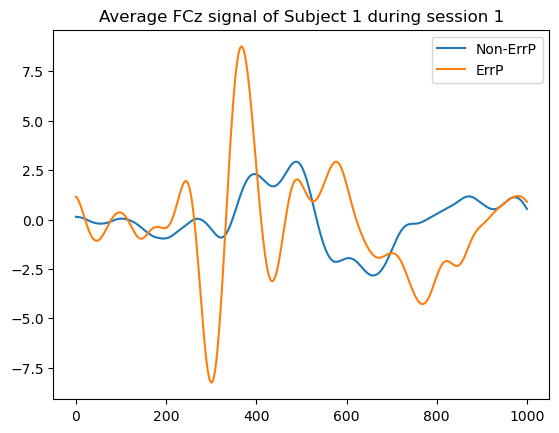
\includegraphics[width=7.7cm]{img/FcZs1s1-1000ms.png}
    \caption{The average non-ErrP and ErrP signal on the FcZ channel. These signals originate from subject 1 during session 1.}
    \label{fig:FcZ}
\end{figure}

Figure \ref{fig:FcZ} shows that the most considerable difference between \verb|ErrP| and \verb|non-ErrP| signals occurs between 200 and 500 milliseconds after the feedback presentation. For this reason, the window size will be 600ms to capture these differences between signals. Note that this graph only shows the FcZ channel, which is the most prominent for ErrP signals.

This window size results in the input EEG data being a matrix of size 64 x 308. The number of rows is the 64 channels of the EEG, and the number of columns is the length of the windows, 600ms of a 512Hz sampling rate.

The decision to feed all 64 channels into the model was made for two reasons. First, previous experiments have shown that feeding all channels instead of pre-selecting electrodes consistently resulted in higher accuracy \citep{correia2021error}. Second, the main aim of this research is to study uncertainty. Using all channels could present more exciting results concerning the amount and origin of uncertainty instead of only using a select amount of channels.

\subsubsection{Balancing}

Due to the nature of the experiment of the used dataset, the data is inherently unbalanced with a 1/5 ratio. Only 20\% of the trials are \verb|ErrP| trials. Rebalancing is necessary to prevent the model from predicting all input episodes as \verb|non-ErrP|. The under-represented class \verb|ErrP| will be over-sampled in the training set until the two classes are represented equally.

The dataset split for the model's training, validation and testing was carefully considered to stick as close as possible to the real-world application of these classifiers. One participant is put aside for the testing set, and the remaining five participants will be used for training. Furthermore, 20 trials are randomly sampled from the training set to be used as a validation set. This results in approximately 66.7\% of the data being used for training, 16.7\% for validation, and 16.7\% for testing, with the latter being a participant the model has not yet seen in training and validation. 


\subsection{Model}

\subsubsection{Model architecture}

The main body of the model architecture consists of a model called EEGNet, a compact convolutional network tailored explicitly for BCI EEG classification \citep{lawhern2018eegnet}. This model consists of two distinct sequential blocks. 

The first block consists of two convolutional steps in sequence. The first layer applies $F_1$ convolutional filters of size (1, 64), which capture the EEG signal at different band-pass frequencies. Setting $F_1$ to half the sampling rate allows for capturing frequency information at 2Hz and above. Next, a \verb|Depthwise Convolution| is applied to learn a spatial filter. After each convolutional layer, batch normalization is applied. Next, an exponential linear unit (ELU) is applied, followed by a Dropout layer to help regularize the model. Lastly, an average pooling layer is used to reduce the sampling rate to a quarter of the original sampling rate.

The second block consists of a Separable Convolution, which is a Depthwise Convolution followed by $F_2$ Pointwise Convolutions. These convolutions help reduce the number of parameters to fit and explicitly decouple the relationship across feature maps. This operation separates the learning of how to summarize individual feature maps in time from how to combine these feature maps optimally. An Average Pooling Layer follows this block to reduce the free parameters in the model.

In the original model, inputs are passed through the two blocks sequentially, followed by a flattened layer. These blocks are followed by a linear layer, which gives the logits of the model's prediction. This output layer is where our model differs from the original mode. Rather than having only one layer returning the classification logits, our model uses two output layers called \verb|heads|. The first head is a linear layer returning the logits representing the \verb|mean| of the prediction. The second head is a linear layer followed by a softplus layer. This head returns logits representing the \verb|variance| of the model. The softplus layer is necessary to make the variance positive.


\subsubsection{Sampling softmax}

The goal is to capture heteroscedastic aleatoric uncertainty in the model. Currently, our model predicts two vectors. One contains the prediction of the mean of both classes. The other contains the prediction of the variance of both classes. To achieve this capture of heteroscedastic aleatoric uncertainty, a method called \verb|Sampling Softmax| is used \citep{kendall2017uncertainties}. With this method, we have to interpret the model as if it had a Gaussian distribution placed over it:
\begin{equation}
    \hat{x}|w \sim \mathcal{N}(f^w, (\sigma^w)^2)
\end{equation}

\begin{equation}
    \hat{p} = Softmax(\hat{x})
\end{equation}

Here, $f^w$ is the output of the mean head with parameters $w$. $\sigma^w$ is the output of the variance head with parameters $w$. The prediction consists of $f^w$, which is corrupted with Gaussian noise with a variance of $\sigma^w$. The corrupted vector is then squashed with the Softmax function to obtain a vector of probabilities.

Ideally, an analytical integral should be taken from this Gaussian Distribution. However, no such solution exists to achieve this. Therefore, an approximation of the integral has to be made. This approximation is achieved through Monte Carlo integration. Here we sample from the aforementioned normal distribution and apply the softmax function to each sample. Using these samples, we can calculate the mean and variance.


\subsubsection{Loss function}

This used architecture raises a question. How can we find the optimal model parameters $\theta$, which results in the most accurate predictions of the mean while simultaneously predicting a variance capturing the aleatoric uncertainty? The loss function should allow the model to reduce the received loss by predicting a high variance on incorrect predictions. However, it is undesirable if the model predicts high variance on all input sequences and thus needs to be punished for predicting high uncertainty on correct predictions. One may ask how this can be achieved. Previous research by \cite{seitzer2022pitfalls} found such a method to achieve this desired behavior. This method is called $\beta$-NLL:

\begin{equation}
    \mathcal{L}_{\beta-NLL} := \underset{X, Y}{\mathbb{E}} \left[ \lfloor \hat{\sigma}^{2\beta}(X) \rfloor NLL \right]
\end{equation}

Here, the $\lfloor. \rfloor$ indicates the \verb|stop gradient| operator. This operator makes $\hat{\sigma}^{2\beta}(X)$ act as a learning rate, which is dependent on the variance prediction. If $\beta$ is set to 0, the loss function behaves like a normal NLL loss. If the value is set to $0.5$, interesting behaviour is observed. Now, all data points are weighted down by $\frac{1}{\sigma}$ (inverse standard deviation instead of inverse variance). Experiments by \cite{seitzer2022pitfalls} showed that $\beta = 0.5$ achieved the best balance between accuracy and log-likelihood.

To find the optimal model parameters $\theta$, the negative log-likelihood (NLL) is used:

\begin{equation}
    NLL := \frac{1}{2}\log \hat{\sigma}^2(X) + \frac{\mathcal{L}_\theta}{\hat{\sigma}^2(X)}
\end{equation}

This loss measures the discrepancy between the predicted and target distributions, assuming a Gaussian distribution with mean $\mu$ and variance $\sigma^2$. Here, the left term $\frac{1}{2}\log \hat{\sigma}^2(X)$ acts as a normalization factor for the NLL loss, which ensures the model learns to predict the best possible mean and variance parameters for the given data. In the right term, $\mathcal{L}_\theta$ is the loss function used nested in the NLL loss. This loss is divided by $\hat{\sigma}^2(X)$. By dividing this loss by the variance, we ensure that the NLL loss is sensitive to the accuracy of the predicted mean $\mu$ and the uncertainty estimation encoded in the predicted variance $\sigma^2$, a higher uncertainty estimation, results in a higher dividing factor, and thus a lower loss. The first term ensures the model does not always predict a high $\sigma^2$.

In the original paper, the task was a regression task, and the used loss function $\mathcal{L}_\theta$ was the mean squared error loss (MSE). In our case, the task at hand is a classification task. For this, we will use the Binary Cross Entropy loss (BCE):

\begin{equation}
    \mathcal{L}_\theta := - ( Y \log \hat{\mu}(X) + (1 - Y) \log (1 - \hat{\mu}(X)) )
\end{equation}

The BCE loss measures the difference between the variable's predicted probability distribution and the variable's true probability distribution. The first term in this function, $Y \log \hat{\mu}(X)$, punishes the model when it predicts a low probability $\mu(X)$ for the positive class. Similarly, the second term punishes the model when it predicts a high probability for the negative class. These two terms ensure that BCE loss penalizes the model for incorrect predictions.

The combination of these three elements allows $\beta$-NLL to ensure that the model learns to predict an optimal mean $\mu$ and variance $\sigma^2$, capturing the aleatoric uncertainty of the model.


\subsection{Explainable AI}

To understand what our model is doing and explain where the uncertainty originates from, we need to introduce a method of Explainable AI to our model. For this, a method based on Shapley values will be used.

\verb|Shapley values| are a concept originating from the cooperative game theory field. They provide a way of allocating a value generated by a group of players to each player. This strategy has been widely adapted to the field of machine learning. They attribute each input feature's contribution to the model's final prediction. This resulting attribution method is called \verb|SHAP| (SHapley Adaptive exPlanations)

The key idea behind SHAP values is to decompose the model's output into the contribution of each input feature while also considering their relations with the other features. Exact calculations are practically impossible to calculate for larger inputs. Instead, the SHAP values are calculated by approximation. This algorithm involves sampling a subset of the features and computing the SHAP values for each sample. The final values are then averaged over all samples to estimate the feature importance.

The advantage of using the SHAP approach is its flexibility and generality. They can be applied to various models, including classification tasks. Moreover, they provide a rich and interpretable representation of the model's behaviour. Another advantage of SHAP values is that we can differentiate between the two heads. Using SHAP, we can build an understanding of how each feature contributed solely to the mean prediction and how they contributed solely to the variance prediction. The latter is of high interest in explaining the origins of the uncertainty. 

\subsection{Experiment design}

This section describes the designs of the three experiments and the training methods used in these experiments.

\subsubsection{Artificial noise}

To properly test whether our suggested approach captures aleatoric uncertainty, we need a method of artificially introducing noise to our data to invoke this uncertainty. Optimally, in the bane of BCIs, we would like to add noise to the data, which frequently occurs on EEG data. However, artificially adding physiological artefacts, such as muscle movements, is beyond our reach and could be an exciting topic for further research. For this paper, we keep the artificial noise simple. The first method of artificial noise generation is adding Gaussian noise to our data. Each data point, within the desired range, will receive noise sampled from a Gaussian distribution of varying intensity. The second method of applying artificial noise is designed to simulate faulty or improperly connected sensors. This method will set a random amount of data points to zero within a specific range.

\begin{figure}[!tbp]
    \centering
        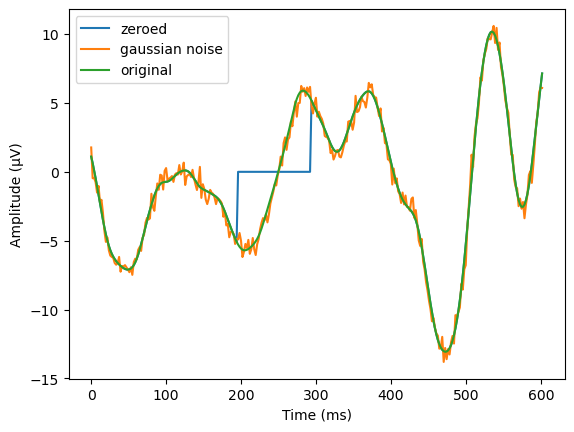
\includegraphics[width=7.7cm]{img/noise.png}
    \caption{FcZ signal with artificially introduced Gaussian noise and localized zeroing.}
    \label{fig:noise}
\end{figure}

Figure \ref{fig:noise} shows an example of artificially generated noise. The green signal is the original FcZ signal, whereas the orange signal has artificially introduced Gaussian noise across the entire signal, with a standard deviation of $0.5$. The blue signal shows an artificial local zeroing between 200 and 250ms.

\subsubsection{Experimental setup}

Each experiment uses the same hyperparameters optimal for EEGNet, suggested by \cite{lawhern2018eegnet}. Each training run will last for 50 epochs. This amount showed to be a good balance between performance and computational time. Each training session is averaged over a total of six runs. Each run uses a different participant as the test participant. The training was done using an NVIDIA GTX 1070 and took around 30 minutes per training session of six runs with 50 epochs each.

\subsubsection{Effect of general noise}

The first experiment adds noise to the entire input length, increasing the noise amount and intensity with every training session. It is expected that the addition of noise should result in a higher overall uncertainty compared to the clean data. The increase in the amount and intensity of the noise between training sessions is also expected to increase the predicted uncertainty between these sessions.

This experiment will accompany a test where labels are shuffled with increasing intensity. Here it is also expected that the uncertainty increases linearly with the number of shuffled labels. 

\subsubsection{Effect of localized noise}

The second experiment will test whether the location of the added noise affects the predicted uncertainty. Two training sessions will be completed here, each with a different input data section corrupted. Both sections have an equal length and intensity of noise. One section will be located on the area with the most contribution to input data, which will be located using the SHAP approximation on the mean head. The second location will be an area with the most minor contribution to the output. Adding noise to the high-contribution areas is expected to result in a more substantial increase in uncertainty than adding noise to the low-contribution areas.

\subsubsection{Tracable noise}

For the final experiment, we test whether we can trace the uncertainty through the SHAP approximation. Here, we add localized noise to some regions of the input data. Afterwards, the SHAP approximation is taken and compared to the SHAP approximation of the original input data. We expect that a shift in the SHAP values is noticeable. Ultimately, the area where we added noise should have higher uncertainty than the other areas and can be located by plotting the SHAP values.